\documentclass{amia}
\usepackage{graphicx}
\usepackage[labelfont=bf]{caption}
\usepackage[superscript,nomove]{cite}
\usepackage{color}


\begin{document}

\noindent{\bf Abstract (50-75 words, do not include in 1-page submission)}

\textit{Through a worked case study of an R package and Shiny dashboard for self-service health authority submission quality duration estimates, we lay a framework for robust efficiency. We make recommendations on 1) transparent, robust and reproducible cohort definitions, 2) defensive restriction of user inputs to maintain results integrity, 3) the importance of separating scientific logic into a documented and tested independent package, 4) and a strategy for clear communication of validation scope and assumptions.}

After the poster session, the learner should be better able to:

\begin{itemize}
  \item Understand the importance of isolating, testing and documenting scientific logic as independent of graphical user interface code
  \item Have an understanding of unit testing and its application to the correct level of units of scientific logic code.
\end{itemize}

\pagebreak

\title{Case study in the development of a framework for quality and reproducibility in inner-sourced packages and self-service analytic dashboards to accelerate common study types}

\author{James A. Black, PhD$^{1}$, Nayan Chaudhary, MSc$^{3}$, Adam J. Foryś, PhD$^{2}$,Sriraman Madhavan, MSc$^{3}$, Matthew Seacrest, MSc$^{3}$, Kamil Wais, PhD$^{2}$} 

\institutes{
    $^1$PD Data Science, Roche, Switzerland; $^2$7N Consulting, Poland; $^3$PD Data Science, Genentech, United States. All authors contributed equally.\\
}

\maketitle

\section*{Introduction and Principles}

Replicability of a research question and reproducibility of individual studies are hampered in studies due to the diversity in the code that sits between a statistical analysis plan and a result. We propose a set principles that can be immediately implemented to boost efficiency. 

\begin{description}
  \item[Code has value:] The use of ad hoc code within a study should be minimised, and a culture promoted of collaboration on pan-study code in documented packages for reuse. Unit tests are ideally written at function creation, and reviewed and expanded with new use cases.
  \item[Democratise access to analytics:] Aided by the consolidation of code into packages, less technical users should be given access to well documented packages to promote guided analyses, as well as dashboards considered for fully self-service interaction.
  \item[Be verbose and specific on input cohorts:] Publish cohort derivation code as user readable markdown vignettes with descriptive statistics and assumption checks.
  \item[Assertively limit user inputs in dashboards:] Developers should ensure that variables exposed for manipulation in the app can be varied without comprimsing validation.
  \item[Separate logic from the user interface:] As shown in Figure ~\ref{fig1}, scientific logic should be separated from visualisation code. This loosely coupled approach improves the robustness of the system by making it easier to isolate, test and document any logic applied to the data.
\end{description}


\begin{figure}[h!]
\centering
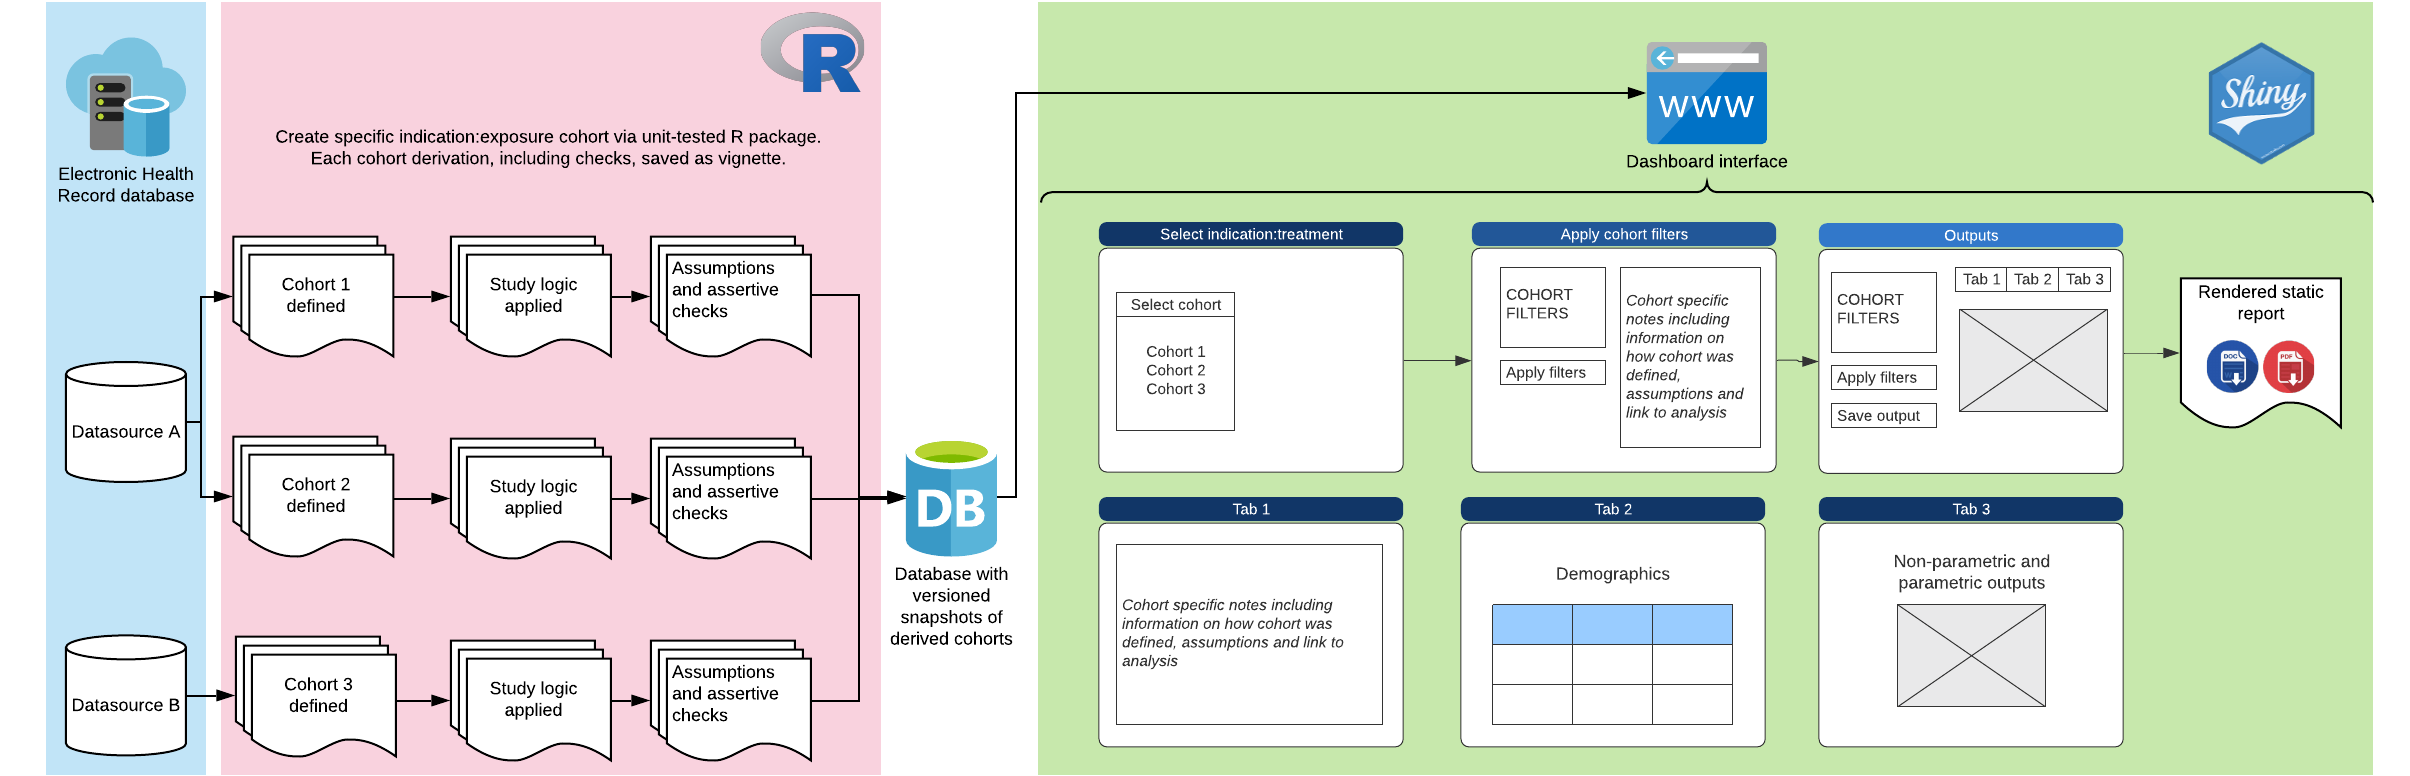
\includegraphics[width=\textwidth]{pics/abstract_image.png}
\caption{Framework for efficiency in running routine study types while maintaining robust and validated results}
\label{fig1}
\end{figure}

\section*{Conclusion}
By applying these principles to a common study data type, the estimation of duration of treatment in real world settings using routinely collected data, we were able to accelerate time to deliver study results from months to days, while improving robustness and standardisation via well documented and tested code.

\end{document}
